% =====================================================================
%  Temporal Accuracy in Rehosted Firmware
%  A Temporal Fidelity Layer for the Renode Emulation Framework
%
%  MSc Thesis — Sandip Kumar Mourya — Saarland University
%
%  Build:  pdflatex -> bibtex -> pdflatex -> pdflatex
%          (or simply upload the docs/thesis folder to Overleaf
%           and set main.tex as the root document)
% =====================================================================
\documentclass[11pt,a4paper,twoside,openright]{report}

% ----- encoding & fonts ----------------------------------------------
\usepackage[utf8]{inputenc}
\usepackage[T1]{fontenc}
\usepackage{lmodern}
\usepackage{microtype}

% ----- page layout ---------------------------------------------------
\usepackage[a4paper,
            inner=3.0cm, outer=2.5cm,
            top=2.5cm, bottom=2.5cm,
            headheight=14pt]{geometry}
\usepackage{setspace}
\onehalfspacing
\usepackage{emptypage}          % no headers/footers on blank pages

% ----- headers -------------------------------------------------------
\usepackage{fancyhdr}
\pagestyle{fancy}
\fancyhf{}
\fancyhead[LE]{\nouppercase{\leftmark}}
\fancyhead[RO]{\nouppercase{\rightmark}}
\fancyfoot[C]{\thepage}
\renewcommand{\headrulewidth}{0.4pt}

% ----- math, units, tables -------------------------------------------
\usepackage{amsmath,amssymb}
\usepackage{siunitx}
\sisetup{range-units=single, per-mode=symbol}
\DeclareSIUnit\sample{S}     % logic-analyser sample
\DeclareSIUnit\baud{Bd}
\DeclareSIUnit\byte{B}
\usepackage{booktabs}
\usepackage{multirow}
\usepackage{array}

% ----- graphics & diagrams -------------------------------------------
\usepackage{graphicx}
\graphicspath{{figures/}}
\usepackage{tikz}
\usetikzlibrary{arrows.meta,positioning,shapes.misc,fit,calc}
\usepackage{caption}
\captionsetup{font=small,labelfont=bf}
\usepackage{subcaption}

% ----- code listings --------------------------------------------------
\usepackage{listings}
\usepackage{xcolor}
\definecolor{codegray}{gray}{0.95}
\definecolor{codecomment}{rgb}{0.30,0.45,0.30}
\definecolor{codekw}{rgb}{0.10,0.15,0.55}
\definecolor{codestr}{rgb}{0.55,0.25,0.10}
\lstset{
  basicstyle=\ttfamily\footnotesize,
  keywordstyle=\color{codekw}\bfseries,
  commentstyle=\color{codecomment}\itshape,
  stringstyle=\color{codestr},
  backgroundcolor=\color{codegray},
  frame=single, framerule=0.2pt, rulecolor=\color{black!25},
  numbers=left, numberstyle=\tiny\color{black!50}, numbersep=6pt,
  breaklines=true, showstringspaces=false, tabsize=4,
  captionpos=b,
  aboveskip=1.0em, belowskip=1.0em
}
\lstdefinelanguage{repl}{
  morekeywords={using,frequency},
  sensitive=false,
  morecomment=[l]{//},
  morestring=[b]"
}
\lstdefinelanguage{resc}{
  morekeywords={mach,create,machine,LoadPlatformDescription,LoadELF,
                start,showAnalyzer,logLevel,using,sysbus,include},
  sensitive=false,
  morecomment=[l]{\#},
  morestring=[b]"
}

% ----- bibliography ---------------------------------------------------
\usepackage[numbers,sort&compress]{natbib}
\bibliographystyle{abbrvnat}

% ----- hyperlinks (load last, cleveref after) --------------------------
\usepackage[hidelinks,
            pdftitle={Temporal Accuracy in Rehosted Firmware},
            pdfauthor={Sandip Kumar Mourya}]{hyperref}
\usepackage[capitalise,noabbrev]{cleveref}

% ----- convenience macros ---------------------------------------------
\newcommand{\TFL}{TFL}
\newcommand{\us}{\si{\micro\second}}
\newcommand{\ns}{\si{\nano\second}}
\newcommand{\ms}{\si{\milli\second}}
\newcommand{\ksleep}{\texttt{k\_sleep()}}
\newcommand{\ktimer}{\texttt{k\_timer}}
\newcommand{\srcS}[1]{\textbf{S#1}}

% =====================================================================
\begin{document}

% ---------------------------------------------------------------------
%  FRONT MATTER
% ---------------------------------------------------------------------
\pagenumbering{roman}
\pagestyle{empty}

% ---------------------------------------------------------------------
%  Title page — Saarland University MSc thesis
% ---------------------------------------------------------------------
\begin{titlepage}
  \centering

  {\Large Saarland University\par}
  {\large Faculty of Mathematics and Computer Science\par}
  {\large Department of Computer Science\par}

  \vspace{2.0cm}

  {\large Master's Thesis\par}

  \vspace{1.2cm}

  \rule{\textwidth}{0.4pt}\par
  \vspace{0.6cm}
  {\LARGE\bfseries Temporal Accuracy in Rehosted Firmware\par}
  \vspace{0.4cm}
  {\large A Temporal Fidelity Layer for the Renode Emulation Framework\par}
  \vspace{0.6cm}
  \rule{\textwidth}{0.4pt}\par

  \vspace{2.0cm}

  {\large submitted by\par}
  \vspace{0.3cm}
  {\Large\bfseries Sandip Kumar Mourya\par}

  \vspace{1.5cm}

  \begin{tabular}{r@{\hspace{1em}}l}
    Supervisor:      & \emph{[Supervisor name]}       \\[0.3em]
    First reviewer:  & \emph{[First reviewer name]}   \\[0.3em]
    Second reviewer: & \emph{[Second reviewer name]}  \\
  \end{tabular}

  \vfill

  {\large Saarbr\"ucken, \today\par}
\end{titlepage}

\cleardoublepage

% ---------------------------------------------------------------------
%  Statement in lieu of an oath / Declaration of consent
%  (standard wording used at Saarland University)
% ---------------------------------------------------------------------
\chapter*{Statement in Lieu of an Oath}

I hereby confirm that I have written this thesis on my own and that I
have not used any other media or materials than the ones referred to in
this thesis.

\vspace{2.5cm}

\noindent
Saarbr\"ucken, \rule{4cm}{0.4pt} \hfill \rule{6cm}{0.4pt}\\
\phantom{Saarbr\"ucken, }(Date) \hfill (Signature)

\vspace{3cm}

\section*{Declaration of Consent}

I agree to make both versions of my thesis (with a passing grade)
accessible to the public by having them added to the library of the
Computer Science Department.

\vspace{2.5cm}

\noindent
Saarbr\"ucken, \rule{4cm}{0.4pt} \hfill \rule{6cm}{0.4pt}\\
\phantom{Saarbr\"ucken, }(Date) \hfill (Signature)

\cleardoublepage

\pagestyle{plain}
% ---------------------------------------------------------------------
%  Abstract
% ---------------------------------------------------------------------
\chapter*{Abstract}
\addcontentsline{toc}{chapter}{Abstract}

Rehosting---executing unmodified embedded firmware inside a full-system
emulator---has become a standard technique for testing, debugging, and
security analysis of embedded software. Frameworks such as Renode
faithfully reproduce the \emph{functional} behaviour of microcontroller
platforms, but their \emph{temporal} behaviour can deviate substantially
from real hardware: emulated clocks advance in coarse scheduling quanta,
interrupt latency is idealised, and physical effects such as oscillator
drift and bus propagation delay are absent entirely. For timing-sensitive
firmware, these deviations can hide real bugs and create false confidence
in test results.

This thesis quantifies and mitigates the temporal deviation between a
physical microcontroller and its rehosted counterpart. Using an
STM32F103RB (Arm Cortex-M3, \SI{72}{\mega\hertz}) running Zephyr RTOS and
an instrumented GPIO-marker firmware, we measure ten timing scenarios on
real hardware with a \SI{100}{\mega\sample\per\second} logic analyser and compare them
against the identical firmware running in Renode~1.15.3. The comparison
reveals systematic deviations of up to three orders of magnitude in
timing \emph{variance}: the emulator is simultaneously too deterministic
for tick-quantised sleeps (jitter ratio ${\approx}\,0.2$) and too noisy
for hardware-timer callbacks (jitter ratio up to $23{\times}$).

Guided by a taxonomy of five deviation sources, we design and implement
the \emph{Temporal Fidelity Layer} (TFL): three composable C\# peripheral
models for Renode---a clock model injecting configurable drift and
Gaussian jitter, a deadline monitor recording task wakeup deviation, and
a bus delay model reproducing inter-node propagation latency. TFL
requires no changes to Renode itself and no changes to the firmware
logic; it is enabled purely through platform description files.

Across seven statistically evaluated scenarios, TFL reduces the
geometric-mean jitter-ratio error from $7.6{\times}$ to $2.9{\times}$
and brings four of seven scenarios within a factor of $1.7$ of hardware
variance. We further characterise the fidelity--performance trade-off of
Renode's scheduling quantum, showing that quantum reduction alone cannot
reach hardware-level fidelity at acceptable simulation cost. All
measurements, models, and analysis scripts are released as open
research artefacts.

\cleardoublepage

% ---------------------------------------------------------------------
%  Acknowledgements
% ---------------------------------------------------------------------
\chapter*{Acknowledgements}
\addcontentsline{toc}{chapter}{Acknowledgements}

I would like to thank my supervisor, \emph{[Supervisor name]}, for the
guidance and feedback throughout this work, and the reviewers for taking
the time to evaluate this thesis.

I am grateful to the Renode and Zephyr open-source communities, whose
documentation and code made this work possible, and to my family and
friends for their constant support during my studies at Saarland
University.

\cleardoublepage

\tableofcontents
\cleardoublepage
\listoffigures
\cleardoublepage
\listoftables
\cleardoublepage

% ---------------------------------------------------------------------
%  MAIN MATTER
% ---------------------------------------------------------------------
\pagenumbering{arabic}
\pagestyle{fancy}

% =====================================================================
\chapter{Introduction}
\label{ch:introduction}
% =====================================================================

\section{Motivation}
\label{sec:intro:motivation}

Embedded systems increasingly control safety- and time-critical
processes: motor controllers, medical devices, automotive electronic
control units, and industrial field buses all depend on firmware that
must react \emph{correctly} and \emph{on time}. Development and
verification of such firmware traditionally requires physical hardware,
which is expensive to scale, difficult to automate, and awkward to
instrument. \emph{Rehosting}---running unmodified firmware binaries
inside a full-system emulator---removes these obstacles and has become
a cornerstone of modern embedded workflows, from continuous-integration
testing~\cite{renode} to large-scale firmware security
analysis~\cite{fasano2021sok,wright2021challenges}.

Emulation frameworks such as Renode~\cite{renode} and
QEMU~\cite{bellard2005qemu} model the \emph{functional} contract of a
microcontroller: instruction semantics, memory maps, peripheral
registers, and interrupt controllers. Firmware that passes functional
tests in the emulator will, in most cases, execute the same logic on
real silicon. The \emph{temporal} contract, however, is a different
matter. Emulators advance virtual time in discrete scheduling quanta,
dispatch interrupts at quantum boundaries, execute instruction blocks at
an idealised rate, and omit analog-world phenomena such as crystal
oscillator drift, temperature-dependent jitter, and bus propagation
delay. As a result, a rehosted firmware image experiences a timing
environment that can differ from the physical one by orders of
magnitude---in either direction.

This discrepancy matters. A control loop that misses its deadline only
under real-world scheduling jitter will appear healthy in the emulator.
Conversely, quantum-induced noise in the emulator can trigger spurious
timeouts that never occur on hardware. In both cases the emulator's
verdict is misleading, undermining the very purpose of rehosted
testing. Despite this, the temporal accuracy of modern rehosting
frameworks has received little systematic, hardware-grounded
quantification.

\section{Problem Statement}
\label{sec:intro:problem}

This thesis addresses two questions:

\begin{enumerate}
  \item \textbf{RQ1 --- Quantification.} How large is the temporal
        deviation between an unmodified firmware image running on a
        physical Arm Cortex-M3 microcontroller and the same image
        rehosted in Renode, across representative RTOS timing
        primitives (sleeps, hardware timers, thread scheduling,
        interrupt service latency), and which mechanisms cause it?
  \item \textbf{RQ2 --- Mitigation.} Can the deviation be reduced by a
        lightweight, non-invasive extension layer---without modifying
        the emulator core, without patching the firmware, and without
        sacrificing the usability that makes rehosting attractive in
        the first place?
\end{enumerate}

\section{Contributions}
\label{sec:intro:contributions}

The thesis makes the following contributions:

\begin{itemize}
  \item \textbf{A measurement methodology and instrumented firmware}
        for comparing physical and virtual timing behaviour. A Zephyr
        RTOS firmware exercises ten timing scenarios and exposes each
        event as a GPIO edge, captured on hardware by a
        \SI{100}{\mega\sample\per\second} logic analyser and in Renode by a GPIO
        tracing hook (\cref{ch:problem}).
  \item \textbf{A taxonomy of five temporal deviation sources}
        (\srcS{1}--\srcS{5}), separating instruction-timing
        abstraction, interrupt delivery latency, clock drift and
        jitter, scheduler quantisation, and inter-node propagation
        delay (\cref{sec:problem:sources}).
  \item \textbf{The Temporal Fidelity Layer (TFL)}, three composable
        Renode peripheral models written in C\# that inject or monitor
        the missing temporal effects: \texttt{TFL\_ClockModel}
        (\srcS{3}), \texttt{TFL\_DeadlineMonitor} (\srcS{4}), and
        \texttt{TFL\_BusDelayModel} (\srcS{5}). TFL attaches purely via
        Renode platform descriptions and works with stock
        Renode~1.15.3 (\cref{ch:design}).
  \item \textbf{A statistical evaluation} of baseline Renode and
        TFL-enhanced Renode against hardware ground truth, including
        distribution comparisons, Mann--Whitney significance tests,
        a quantum-sensitivity study, and a workload-interference study
        (\cref{ch:evaluation}).
  \item \textbf{Open research artefacts}: firmware, peripheral models,
        platform files, capture data, and the full analysis pipeline
        are available in the accompanying repository
        (\cref{app:reproducibility}).
\end{itemize}

\section{Thesis Outline}
\label{sec:intro:outline}

\cref{ch:background} introduces the technical background on embedded
timing, the STM32F103 platform, Zephyr RTOS, and the Renode emulation
framework. \cref{ch:relatedwork} surveys related work on rehosting and
timing-accurate simulation. \cref{ch:problem} develops the measurement
methodology and the deviation-source taxonomy, and presents the
baseline characterisation of Renode against hardware.
\cref{ch:design} describes the design and implementation of the
Temporal Fidelity Layer. \cref{ch:evaluation} evaluates TFL
quantitatively. \cref{ch:conclusion} concludes and outlines future
work.

% =====================================================================
\chapter{Background}
\label{ch:background}
% =====================================================================

\section{Timing in Embedded Systems}
\label{sec:bg:timing}

Embedded firmware interacts with the physical world through deadlines:
a PWM edge must occur every control period, a sensor must be sampled at
a fixed rate, a bus frame must be acknowledged within a protocol
timeout. Two properties characterise the timing behaviour of such a
system:

\begin{description}
  \item[Accuracy] --- how close the \emph{mean} of an observed interval
        is to its nominal value (e.g.\ a \SI{10}{\milli\second} timer
        firing every \SI{10.001}{\milli\second} on average).
  \item[Jitter] --- the \emph{variance} of the interval around its
        mean, typically reported as a standard deviation or a
        percentile bound.
\end{description}

Real microcontrollers derive their notion of time from a crystal or RC
oscillator whose frequency exhibits static offset (specified in parts
per million, ppm), temperature drift, and cycle-to-cycle jitter. On top
of this physical layer, the RTOS adds software-induced timing effects:
tick quantisation, scheduling latency, priority inversion, and
interrupt masking windows. Any faithful emulation of firmware timing
must account for both layers.

\section{The Target Platform: STM32F103RB and Zephyr RTOS}
\label{sec:bg:platform}

All experiments in this thesis use the ST NUCLEO-F103RB development
board. Its STM32F103RB microcontroller~\cite{stm32rm0008} integrates an
Arm Cortex-M3 core~\cite{armcm3trm} clocked at \SI{72}{\mega\hertz},
\SI{20}{\kilo\byte} SRAM, and \SI{128}{\kilo\byte} flash. Three
properties make it a good measurement target:

\begin{itemize}
  \item The Cortex-M3 has a well-documented, deterministic interrupt
        model with a minimum interrupt latency of 12 cycles
        (\SI{167}{\nano\second} at \SI{72}{\mega\hertz})~\cite{armcm3trm}.
  \item The Data Watchpoint and Trace (DWT) unit provides a free-running
        CPU cycle counter (\texttt{DWT\_CYCCNT}), enabling
        cycle-granular self-instrumentation.
  \item The platform is fully supported by both Zephyr and Renode,
        allowing bit-identical firmware to run in both environments.
\end{itemize}

The firmware is built on Zephyr RTOS~3.6.0~\cite{zephyr}, a
widely-deployed open-source RTOS. Zephyr's kernel timing primitives
used in this work are:

\begin{itemize}
  \item \ksleep{} --- suspends the calling thread for a given number of
        ticks. With the default \SI{1000}{\hertz} tick rate, requested
        durations are rounded \emph{up} to the next tick boundary,
        introducing a systematic $0$--$1$\,\ms{} quantisation delay.
  \item \texttt{k\_busy\_wait()} --- spins on the cycle counter without
        yielding, providing sub-tick delays.
  \item \ktimer{} --- hardware-timer-backed periodic callbacks,
        dispatched from the system clock interrupt independent of the
        scheduler tick.
  \item Thread scheduling --- preemptive, priority-based scheduling
        with optional time slicing.
\end{itemize}

\section{Firmware Rehosting}
\label{sec:bg:rehosting}

Rehosting (also \emph{re-hosting} or firmware emulation) denotes the
execution of firmware compiled for an embedded target inside a
software environment on a host machine~\cite{fasano2021sok}. Depending
on how much of the hardware is modelled, approaches range from
high-level API interception (HALucinator~\cite{clements2020halucinator})
over automatically inferred peripheral models
(P$^2$IM~\cite{feng2020p2im}, Pretender~\cite{gustafson2019pretender},
$\mu$Emu~\cite{zhou2021uemu}) to full-system emulation with hand-written
peripheral models (QEMU~\cite{bellard2005qemu}, Renode~\cite{renode}).
Full-system emulation offers the strongest fidelity guarantees for
\emph{functional} behaviour because the unmodified binary executes
against a complete register-level model of the SoC.

\section{The Renode Emulation Framework}
\label{sec:bg:renode}

Renode~\cite{renode} is an open-source emulation framework by Antmicro,
targeted specifically at embedded and multi-node IoT systems. Its
architecture is relevant to this thesis in four respects.

\paragraph{Platform descriptions.} A machine is assembled from a
\texttt{.repl} (Renode platform) file that instantiates peripherals at
bus addresses. Peripherals are C\# classes loaded at runtime; users can
add custom peripherals \emph{without recompiling Renode}. This
extension mechanism is the foundation of the Temporal Fidelity Layer.

\paragraph{Translation-based CPU emulation.} Guest instructions are
executed through a translation library derived from tlibs. Renode does
not simulate microarchitectural effects (pipeline, caches, flash wait
states); instead, each CPU is assigned a nominal performance in MIPS
(here: 72), and executed instruction counts are converted into virtual
time at that fixed rate. Deviation source \srcS{1}
(\cref{sec:problem:sources}) follows directly from this abstraction.

\paragraph{Quantum-based virtual time.} Virtual time advances in
discrete slices called \emph{quanta} (default \SI{100}{\micro\second}).
Each CPU executes up to one quantum's worth of instructions before
synchronising with the emulation's master clock. Timer interrupts,
inter-peripheral events, and cross-machine messages are therefore
aligned to quantum boundaries, which quantises event timing
(source \srcS{4}).

\paragraph{Deterministic execution.} Given identical inputs, a Renode
simulation is deterministic: there is no analog noise, no oscillator
drift (source \srcS{3}), and no physical transmission delay between
emulated nodes (source \srcS{5}). Determinism is desirable for
reproducible debugging, but it is precisely the property that separates
emulated timing from physical timing.

\section{Measurement Instrumentation}
\label{sec:bg:instrumentation}

On physical hardware, firmware-internal events are made externally
observable by toggling GPIO pins, captured with a Saleae Logic~8
analyser~\cite{saleae} at \SI{100}{\mega\sample\per\second} (\SI{10}{\nano\second}
resolution). GPIO instrumentation was chosen over trace units (ITM/ETM)
because the identical mechanism exists in Renode: the emulated GPIO
port is hooked to log state changes with virtual-time timestamps,
yielding structurally identical traces from both worlds. The
instrumentation cost itself is quantified in
\cref{sec:eval:instrumentation}.

% =====================================================================
\chapter{Related Work}
\label{ch:relatedwork}
% =====================================================================

\section{Firmware Rehosting and Emulation}
\label{sec:rw:rehosting}

The systematisation by Fasano et al.~\cite{fasano2021sok} and the
survey by Wright et al.~\cite{wright2021challenges} map the design
space of rehosting and identify \emph{fidelity} as its central
challenge. Both works focus predominantly on \emph{execution} fidelity
(does the firmware run at all, and does it take the same paths?) and
\emph{memory/peripheral} fidelity; temporal fidelity is acknowledged
but not quantified. This thesis fills that gap with hardware-grounded
measurements.

Firmadyne~\cite{chen2016firmadyne} pioneered large-scale emulation of
Linux-based firmware; HALucinator~\cite{clements2020halucinator}
replaces hardware-abstraction-layer functions with host-side handlers;
P$^2$IM~\cite{feng2020p2im}, Pretender~\cite{gustafson2019pretender},
and $\mu$Emu~\cite{zhou2021uemu} infer peripheral behaviour
automatically to keep firmware running. All of these systems evaluate
success as ``firmware executes correctly'', with no claim about
\emph{when} events happen. Muench et al.~\cite{muench2018you}
demonstrate that even memory-corruption effects differ between
emulated and physical embedded targets---an early warning that
emulation platforms are not behaviourally transparent. Our work extends
this observation to the time domain.

\section{Timing-Accurate Simulation}
\label{sec:rw:timing}

At the opposite end of the fidelity spectrum, cycle-accurate simulators
model microarchitectural state per clock cycle. gem5~\cite{binkert2011gem5}
provides cycle-approximate CPU models for architecture research, and
commercial virtual platforms such as Simics~\cite{magnusson2002simics}
offer configurable timing models. SystemC/TLM-2.0~\cite{systemc} defines
loosely- and approximately-timed modelling styles in which
transaction-level models annotate delays. These approaches achieve high
temporal fidelity at the cost of simulation speed (typically
$10^2$--$10^5\times$ slower than real time) and modelling effort; they
are rarely practical for full-firmware CI workflows. The Temporal
Fidelity Layer targets the middle ground: statistical (rather than
cycle-exact) timing realism at near-native emulation speed.

\section{Emulator Time Management}
\label{sec:rw:quantum}

QEMU's icount mode~\cite{bellard2005qemu} maps executed instructions to
virtual time at a fixed rate, analogous to Renode's MIPS-based model,
and shares its limitation: instruction counts, not microarchitectural
cycles, drive the clock. Renode's quantum-based synchronisation of
multiple machines~\cite{renode} enables deterministic multi-node
simulation but aligns all cross-machine communication to quantum
boundaries. The evaluation in \cref{sec:eval:quantum} quantifies the
fidelity--performance trade-off of this quantum for the first time on
a hardware-validated workload.

\section{Positioning of this Thesis}
\label{sec:rw:positioning}

To the best of our knowledge, this thesis provides the first
systematic, statistically evaluated comparison of RTOS-level timing
primitives between a physical Cortex-M platform and its rehosted
counterpart in Renode, together with a non-invasive mitigation layer.
Unlike cycle-accurate simulation, TFL does not attempt to reproduce
\emph{individual} event times; it aims to reproduce hardware-like
timing \emph{distributions}---sufficient for testing timing-robustness
of firmware---while preserving emulation speed and determinism controls.

% =====================================================================
\chapter{Problem Analysis and Measurement Methodology}
\label{ch:problem}
% =====================================================================

This chapter answers RQ1. It first develops a taxonomy of the
mechanisms by which rehosted timing deviates from physical timing
(\cref{sec:problem:sources}), then presents the measurement
methodology (\cref{sec:problem:methodology}) and the test scenarios
(\cref{sec:problem:scenarios}) used to quantify each mechanism.

\section{Sources of Temporal Deviation}
\label{sec:problem:sources}

We classify the deviation between emulated and physical timing into
five sources, summarised in \cref{tab:sources}.

\begin{table}[tb]
  \centering
  \caption[Taxonomy of temporal deviation sources]{Taxonomy of temporal
    deviation sources between physical execution and rehosted execution
    in Renode, and the TFL component addressing each source.}
  \label{tab:sources}
  \small
  \begin{tabular}{@{}clll@{}}
    \toprule
    ID & Source & Mechanism in Renode & Addressed by \\
    \midrule
    \srcS{1} & Instruction timing        & Fixed MIPS rate, no $\mu$arch model    & --- (out of scope) \\
    \srcS{2} & Interrupt delivery        & Aligned to translation-block/quantum    & --- (quantified) \\
    \srcS{3} & Clock drift \& jitter     & Ideal oscillator, no noise             & \texttt{TFL\_ClockModel} \\
    \srcS{4} & Scheduler quantisation    & Events snap to \SI{100}{\micro\second} quantum & \texttt{TFL\_DeadlineMonitor} \\
    \srcS{5} & Inter-node propagation    & Zero-delay message delivery             & \texttt{TFL\_BusDelayModel} \\
    \bottomrule
  \end{tabular}
\end{table}

\paragraph{\srcS{1} --- Instruction-timing abstraction.}
Renode converts executed instruction counts to virtual time at a
configured rate (\texttt{PerformanceInMips 72}). Pipeline stalls, flash
wait states, and bus contention on the real Cortex-M3 are not modelled,
so code segments have proportionally distorted durations. Correcting
\srcS{1} requires microarchitectural simulation and is explicitly out
of scope; its magnitude is bounded experimentally via busy-wait tests.

\paragraph{\srcS{2} --- Interrupt delivery latency.}
On hardware, the NVIC preempts within 12 cycles plus bus-dependent
overhead, producing a tight latency distribution (measured
$\sigma \approx \SI{0.9}{\micro\second}$ at RTOS level). In Renode,
interrupts are recognised at translation-block boundaries within a
quantum, yielding a latency distribution governed by block length and
quantum size rather than by the NVIC.

\paragraph{\srcS{3} --- Clock drift and jitter.}
A real crystal oscillator exhibits ppm-scale frequency offset and
temperature drift; the emulated clock is mathematically exact. Any
firmware that calibrates against wall-clock time, synchronises across
nodes, or accumulates time over long horizons behaves unrealistically
optimistically in the emulator.

\paragraph{\srcS{4} --- Scheduler quantisation.}
All virtual-time events are aligned to the emulation quantum (default
\SI{100}{\micro\second}). Timer callbacks that jitter by
$\sigma \approx \SI{1.3}{\micro\second}$ on hardware jitter by
$\sigma \approx \SI{29}{\micro\second}$ in the emulator---a
$23\times$ inflation (\cref{sec:eval:timer})---while tick-quantised
sleeps lose the hardware's inherent $0$--$1$\,\ms{} rounding variance
and appear \emph{too} deterministic.

\paragraph{\srcS{5} --- Inter-node propagation delay.}
Renode delivers messages between emulated machines in zero virtual
time, whereas a physical UART byte at \SI{115200}{\baud} occupies
$\approx \SI{86.8}{\micro\second}$ on the wire. Protocol
implementations tested against zero-latency links can harbour latent
race conditions.

\section{Measurement Methodology}
\label{sec:problem:methodology}

\begin{figure}[tb]
  \centering
  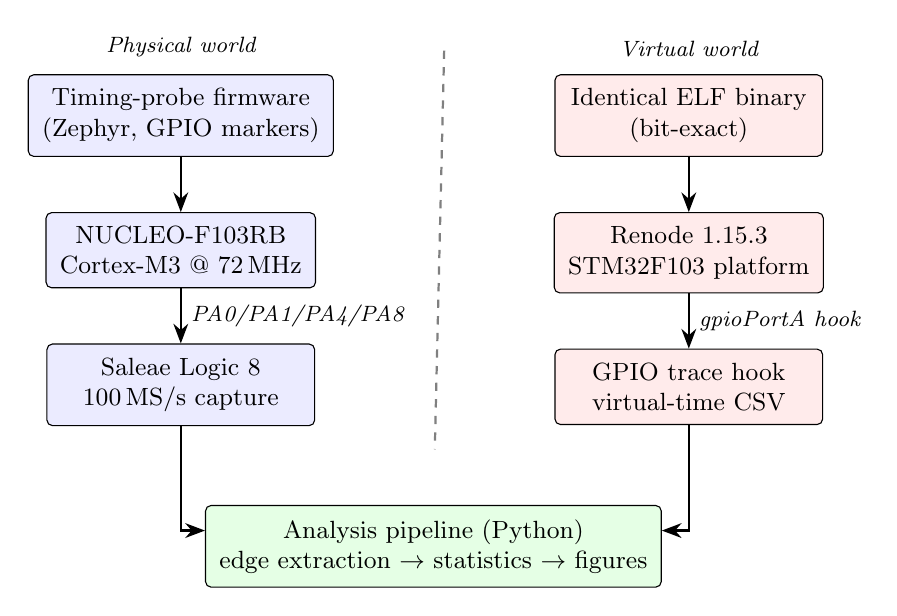
\begin{tikzpicture}[
      font=\small,
      box/.style={draw, rounded corners=2pt, align=center,
                  minimum height=9mm, inner sep=5pt},
      lbl/.style={font=\footnotesize\itshape},
      arr/.style={-{Stealth[length=2.5mm]}, thick}
    ]
    % ---- physical branch ----
    \node[box, fill=blue!8, minimum width=34mm] (fw1)
      {Timing-probe firmware\\ (Zephyr, GPIO markers)};
    \node[box, fill=blue!8, below=7mm of fw1, minimum width=34mm] (hw)
      {NUCLEO-F103RB\\ Cortex-M3 @ 72\,MHz};
    \node[box, fill=blue!8, below=7mm of hw, minimum width=34mm] (la)
      {Saleae Logic 8\\ 100\,MS/s capture};

    % ---- virtual branch ----
    \node[box, fill=red!8, right=28mm of fw1, minimum width=34mm] (fw2)
      {Identical ELF binary\\ (bit-exact)};
    \node[box, fill=red!8, below=7mm of fw2, minimum width=34mm] (ren)
      {Renode 1.15.3\\ STM32F103 platform};
    \node[box, fill=red!8, below=7mm of ren, minimum width=34mm] (gpiolog)
      {GPIO trace hook\\ virtual-time CSV};

    % ---- analysis ----
    \node[box, fill=green!10, minimum width=44mm,
          below right=10mm and -14mm of la] (ana)
      {Analysis pipeline (Python)\\ edge extraction $\to$ statistics $\to$ figures};

    \draw[arr] (fw1) -- (hw);
    \draw[arr] (hw) -- node[lbl, right] {PA0/PA1/PA4/PA8} (la);
    \draw[arr] (fw2) -- (ren);
    \draw[arr] (ren) -- node[lbl, right] {gpioPortA hook} (gpiolog);
    \draw[arr] (la.south) |- ($(ana.west)+(-3mm,2mm)$) -- ($(ana.west)+(0,2mm)$);
    \draw[arr] (gpiolog.south) |- ($(ana.east)+(3mm,2mm)$) -- ($(ana.east)+(0,2mm)$);
    \draw[thick, dashed, gray]
      ($(fw1.north east)!0.5!(fw2.north west)+(0,3mm)$) --
      ($(la.south east)!0.5!(gpiolog.south west)+(0,-3mm)$);
    \node[lbl, above=1mm of fw1] {Physical world};
    \node[lbl, above=1mm of fw2] {Virtual world};
  \end{tikzpicture}
  \caption[Measurement setup]{Measurement setup. The identical firmware
    ELF runs on the physical board and in Renode; GPIO events are
    captured by a logic analyser (physical) and a trace hook (virtual)
    and compared by a common analysis pipeline.}
  \label{fig:setup}
\end{figure}

\Cref{fig:setup} shows the twin measurement paths. Three principles
guarantee comparability:

\begin{enumerate}
  \item \textbf{Bit-identical firmware.} The same
        \texttt{zephyr.elf}, built once with Zephyr SDK~0.16.8, is
        flashed to the board and loaded into Renode. There are no
        emulator-specific code paths.
  \item \textbf{A common observable.} Every timing event is a GPIO edge
        on one of four marker pins (\cref{tab:pinmap} in
        \cref{app:hardware}). Physical edges are timestamped at
        \SI{10}{\nano\second} resolution by the logic analyser; virtual
        edges are timestamped in virtual time by a hook on the emulated
        GPIO port.
  \item \textbf{A common analysis pipeline.} Both trace formats are
        reduced to identical interval series and processed by the same
        statistics code, eliminating tool-induced bias.
\end{enumerate}

\paragraph{Metrics.} For each scenario we report the interval mean
$\mu$, standard deviation $\sigma$, the systematic error
$\mu - T_{\mathrm{nom}}$ against the nominal period, and the
\emph{jitter ratio}
\begin{equation}
  J \;=\; \frac{\sigma_{\mathrm{emu}}}{\sigma_{\mathrm{hw}}},
  \label{eq:jitterratio}
\end{equation}
which equals $1$ for perfect variance fidelity, $J<1$ for an emulator
that is unrealistically deterministic, and $J>1$ for one that is
unrealistically noisy. Because timing distributions are generally
non-Gaussian (verified by Shapiro--Wilk tests~\cite{shapiro1965}),
distribution equality is tested with the non-parametric
Mann--Whitney~$U$ test~\cite{mann1947} at $\alpha=0.01$, with the
rank-biserial correlation $r$ as effect size.

\section{Test Scenarios}
\label{sec:problem:scenarios}

The timing-probe firmware sequences ten scenarios
(\cref{tab:scenarios}), grouped into four categories that isolate
different deviation sources. Each scenario is announced over UART and
delimited by an envelope marker (PA1), sub-tests are separated by
counting pulses on PA4, and the measured event itself toggles PA0.

\begin{table}[tb]
  \centering
  \caption[Timing test scenarios]{Timing test scenarios implemented in
    the probe firmware. Scenarios marked $\dagger$ are used for the
    statistical evaluation in \cref{ch:evaluation}; the remaining
    scenarios serve calibration and plausibility checks.}
  \label{tab:scenarios}
  \small
  \begin{tabular}{@{}llll@{}}
    \toprule
    ID & Scenario & Primitive & Isolates \\
    \midrule
    T1$^\dagger$ & Periodic toggle \SI{1}{\milli\second}   & \ksleep{}            & \srcS{4} tick quantisation \\
    T2$^\dagger$ & Periodic toggle \SI{10}{\milli\second}  & \ksleep{}            & \srcS{4} tick quantisation \\
    T3$^\dagger$ & Periodic toggle \SI{100}{\milli\second} & \ksleep{}            & \srcS{4} tick quantisation \\
    T4 & Busy-wait accuracy sweep                          & \texttt{k\_busy\_wait()} & \srcS{1} instruction timing \\
    T5 & Sleep accuracy sweep                              & \ksleep{}            & \srcS{4} \\
    T6$^\dagger$ & Timer callback jitter \SI{10}{\milli\second} & \ktimer{}       & \srcS{2}/\srcS{4} \\
    T7$^\dagger$ & Thread scheduling jitter                & semaphore wakeup     & \srcS{4} \\
    T8$^\dagger$ & Multi-thread interference               & 3 competing threads  & \srcS{4} \\
    T9$^\dagger$ & ISR latency                             & EXTI interrupt       & \srcS{2} \\
    T10 & Workload impact sweep                            & \ktimer{} + load     & \srcS{2}/\srcS{4} \\
    \bottomrule
  \end{tabular}
\end{table}

\paragraph{Sample sizes.} Fast scenarios (T1, T9) collect 2\,500
intervals per environment; slower scenarios collect 250 (T2, T6--T8)
or 25 (T3) intervals, bounded by capture memory and simulation
wall-clock budget. All reported significance tests are computed on the
full per-scenario sample.

\section{Baseline Characterisation}
\label{sec:problem:baseline}

Applying the methodology to stock Renode~1.15.3 yields the baseline
picture developed in detail in \cref{ch:evaluation}; two findings
motivate the design of TFL and are previewed here.

First, deviations are \emph{bidirectional}. For tick-quantised sleeps
(T1--T3), hardware exhibits $\sigma \approx \SI{400}{\micro\second}$
(dominated by Zephyr's $0$--$1$\,\ms{} tick rounding interacting with
asynchronous test phases), while Renode reproduces only
$\sigma \approx \SI{70}{}$--$\SI{84}{\micro\second}$: jitter ratios of
$0.17$--$0.21$. For hardware-timer callbacks (T6) the situation
inverts: $\sigma_{\mathrm{hw}} = \SI{1.3}{\micro\second}$ versus
$\sigma_{\mathrm{emu}} = \SI{29.4}{\micro\second}$, a jitter ratio of
$23.4$. A single global ``speed-up/slow-down'' correction therefore
cannot fix temporal fidelity; source-specific modelling is required.

Second, mean-level accuracy and variance-level fidelity are
independent failures. In T1--T3 the emulated \emph{means} are within
\SI{0.1}{\percent} of nominal while hardware means carry the
$+1$\,\ms{} tick-rounding offset---so the emulator is ``more accurate''
than reality in the mean, yet completely misses the distribution shape
($p < 10^{-8}$, $|r| > 0.99$ for T1--T3). Fidelity, not idealised
accuracy, is the correct target for rehosted testing.

% =====================================================================
\chapter{The Temporal Fidelity Layer}
\label{ch:design}
% =====================================================================

This chapter answers RQ2 by design. \Cref{sec:design:goals} derives
design goals from the baseline characterisation;
\cref{sec:design:architecture} presents the architecture;
\cref{sec:design:components} details the three components; and
\cref{sec:design:integration} shows how TFL integrates into an
unmodified Renode installation.

\section{Design Goals}
\label{sec:design:goals}

\begin{description}
  \item[G1 --- Non-invasiveness.] No modification of the Renode code
        base and no recompilation: TFL must load into stock
        Renode~1.15.3 at runtime.
  \item[G2 --- Firmware transparency.] The firmware logic under test
        must not change. (The probe firmware writes to optional TFL
        registers for \emph{monitoring}, but these writes are
        no-ops on hardware-only builds and do not alter control flow.)
  \item[G3 --- Statistical realism.] TFL targets distribution-level
        fidelity: emulated timing variance should match hardware
        variance ($J \to 1$ in \cref{eq:jitterratio}), not individual
        event times.
  \item[G4 --- Configurability and reproducibility.] All temporal
        parameters (drift, jitter, delay) are set declaratively in the
        platform description; randomness draws from Renode's seeded
        PRNG so that runs remain reproducible.
  \item[G5 --- Composability.] Each deviation source is modelled by an
        independent component; any subset can be enabled for ablation
        studies.
\end{description}

\section{Architecture}
\label{sec:design:architecture}

\begin{figure}[tb]
  \centering
  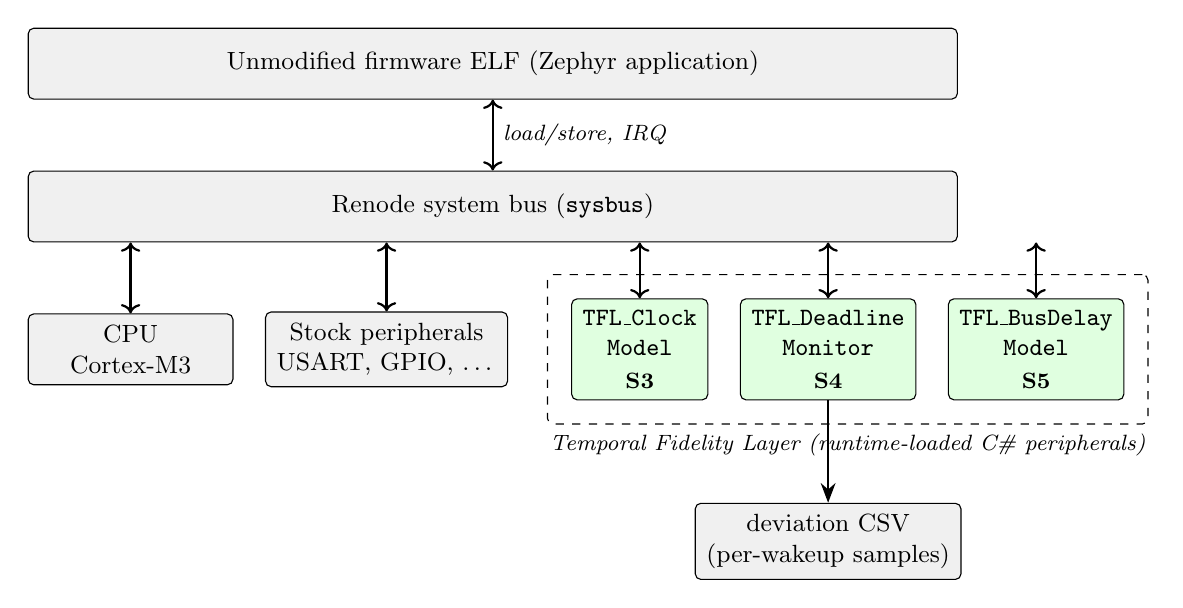
\begin{tikzpicture}[
      font=\small,
      box/.style={draw, rounded corners=2pt, align=center,
                  minimum height=9mm, inner sep=4pt},
      tfl/.style={box, fill=green!12},
      std/.style={box, fill=black!6},
      arr/.style={-{Stealth[length=2.5mm]}, thick},
      lbl/.style={font=\footnotesize\itshape}
    ]
    % firmware
    \node[std, minimum width=118mm] (fw)
      {Unmodified firmware ELF (Zephyr application)};

    % system bus
    \node[std, minimum width=118mm, below=9mm of fw] (bus)
      {Renode system bus (\texttt{sysbus})};

    \draw[arr, <->] (fw) -- node[lbl, right] {load/store, IRQ} (bus);

    % standard peripherals
    \node[std, below=9mm of bus.south west, anchor=north west,
          minimum width=26mm] (cpu) {CPU\\ Cortex-M3};
    \node[std, right=4mm of cpu, minimum width=26mm] (per)
      {Stock peripherals\\ USART, GPIO, \dots};

    % TFL peripherals
    \node[tfl, right=8mm of per, minimum width=17mm] (clk)
      {\texttt{TFL\_Clock}\\ \texttt{Model}\\[1pt] {\footnotesize\srcS{3}}};
    \node[tfl, right=4mm of clk, minimum width=17mm] (mon)
      {\texttt{TFL\_Deadline}\\ \texttt{Monitor}\\[1pt] {\footnotesize\srcS{4}}};
    \node[tfl, right=4mm of mon, minimum width=17mm] (busd)
      {\texttt{TFL\_BusDelay}\\ \texttt{Model}\\[1pt] {\footnotesize\srcS{5}}};

    \draw[arr, <->] (cpu.north) -- ($(cpu.north|-bus.south)$);
    \draw[arr, <->] (per.north) -- ($(per.north|-bus.south)$);
    \draw[arr, <->] (clk.north) -- ($(clk.north|-bus.south)$);
    \draw[arr, <->] (mon.north) -- ($(mon.north|-bus.south)$);
    \draw[arr, <->] (busd.north) -- ($(busd.north|-bus.south)$);

    % TFL brace
    \node[draw, dashed, rounded corners=2pt, fit=(clk)(mon)(busd),
          inner sep=3mm, label={[lbl]below:Temporal Fidelity Layer
          (runtime-loaded C\# peripherals)}] {};

    % csv output
    \node[std, below=13mm of mon, minimum width=30mm] (csv)
      {deviation CSV\\ (per-wakeup samples)};
    \draw[arr] (mon.south) -- (csv.north);
  \end{tikzpicture}
  \caption[TFL architecture]{TFL architecture. The three TFL components
    are ordinary memory-mapped peripherals attached to the system bus by
    the platform description; Renode itself is unmodified.}
  \label{fig:tfl-arch}
\end{figure}

\Cref{fig:tfl-arch} shows the architecture. Each TFL component is a C\#
class deriving from Renode's \texttt{BasicDoubleWordPeripheral},
registered on the system bus by the \texttt{.repl} platform file. Two
integration idioms are used:

\begin{itemize}
  \item \textbf{Shadowing}: \texttt{TFL\_ClockModel} is mapped over the
        SysTick register window (\texttt{0xE000E010}--\texttt{0xE000E02F}),
        transparently perturbing every counter read the firmware
        performs. No firmware cooperation is needed.
  \item \textbf{Side-band}: \texttt{TFL\_DeadlineMonitor} and
        \texttt{TFL\_BusDelayModel} occupy otherwise-unused address
        ranges (\texttt{0x50000000}, \texttt{0x50001000}). Firmware may
        write to them for monitoring (a single \texttt{TFL\_MARK()}
        store, compiled to one \texttt{str} instruction), which is
        harmless on hardware where the region is unmapped\footnote{On
        Cortex-M3 the region is write-ignored in the probe
        configuration; guarding the macro with a build flag is equally
        possible.}.
\end{itemize}

\section{Components}
\label{sec:design:components}

\subsection{TFL\_ClockModel: Drift and Jitter Injection (\srcS{3})}
\label{sec:design:clock}

The clock model exposes a SysTick-compatible register block
(\texttt{CTRL}, \texttt{LOAD}, \texttt{CURRENT}, \texttt{CALIB}). On
every read of \texttt{CURRENT} it computes the ideal cycle count
$c_{\mathrm{true}}$ from virtual time and the configured CPU frequency
$f$, then returns a perturbed value
%
\begin{equation}
  c \;=\; c_{\mathrm{true}}
        \;+\; \underbrace{c_{\mathrm{true}}\cdot
              \frac{D}{10^6}}_{\text{drift, } D~\mathrm{ppm}}
        \;+\; \underbrace{z \cdot \sigma_J \cdot
              \frac{f}{10^9}}_{\text{jitter, } z\sim\mathcal{N}(0,1)},
  \label{eq:clockmodel}
\end{equation}
%
where $D$ (\texttt{DriftPpm}) models static oscillator offset and
$\sigma_J$ (\texttt{JitterNs}) models cycle-to-cycle noise, generated
by a Box--Muller transform from Renode's seeded PRNG (goal G4). The
evaluation configuration uses $D = 25$\,ppm and
$\sigma_J = \SI{150}{\nano\second}$, values within the tolerance band
of the STM32F103's HSE crystal circuit~\cite{stm32rm0008}.

\subsection{TFL\_DeadlineMonitor: Wakeup Deviation Tracking (\srcS{4})}
\label{sec:design:monitor}

The deadline monitor quantifies scheduler-induced deviation
\emph{inside} the emulation. Firmware writes to its \texttt{MARK}
register at every periodic wakeup; the peripheral timestamps the write
in virtual time, computes the deviation from the configured
\texttt{ExpectedPeriodNs}, updates the \texttt{LAST\_DEV\_HI/LO}
registers (readable by the firmware itself, enabling self-adaptive
tests), and streams per-sample records to a CSV file for offline
analysis. This turns the emulator into its own measurement instrument
and provides the virtual-side ground truth used in
\cref{sec:eval:tfl}.

\subsection{TFL\_BusDelayModel: Propagation Delay Injection (\srcS{5})}
\label{sec:design:bus}

The bus delay model provides a \texttt{SEND}/\texttt{RECV} register
pair backed by a bounded delay queue. A value written to \texttt{SEND}
becomes visible at \texttt{RECV} only after
%
\begin{equation}
  t_{\mathrm{deliver}} \;=\; t_{\mathrm{send}} + d + z\cdot\sigma_A,
  \qquad z\sim\mathcal{N}(0,1),
\end{equation}
%
where $d$ (\texttt{PropagationDelayNs}) is the deterministic
propagation delay and $\sigma_A$ (\texttt{ArbitrationJitterNs}) models
arbitration variance. The default $d = \SI{86806}{\nano\second}$ equals
one UART frame (10 bits) at \SI{115200}{\baud}, the wire latency that
stock Renode collapses to zero. \texttt{STATUS} exposes queue depth,
and overflow beyond \texttt{MaxQueueDepth} drops messages and counts
them in \texttt{STATS\_DROP}---reproducing the lossy behaviour of real
buffered links.

\section{Integration and Usage}
\label{sec:design:integration}

TFL is enabled entirely declaratively.
\Cref{lst:repl} shows the complete TFL platform description used in the
evaluation; \cref{lst:resc} shows the corresponding Renode script. An
ablation configuration (clock-only, deadline-only, bus-only) is a
three-line edit, satisfying goal G5.

\begin{lstlisting}[language=repl, caption={TFL platform description
  (\texttt{platforms/nucleo\_f103rb\_tfl.repl}). The base STM32F103
  description is included unchanged; TFL components are added at
  dedicated addresses.}, label={lst:repl}]
using "platforms/cpus/stm32f103.repl"

tfl_clock: Timers.TFL_ClockModel @ sysbus <0xE000E010, 0xE000E02F>
    frequency: 72000000
    DriftPpm:  25.0
    JitterNs:  150.0

tfl_monitor: Miscellaneous.TFL_DeadlineMonitor @ sysbus <0x50000000, 0x5000000F>
    ExpectedPeriodNs: 1000000
    MaxSamples: 10000

tfl_bus: Miscellaneous.TFL_BusDelayModel @ sysbus <0x50001000, 0x5000101F>
    PropagationDelayNs: 86806
    ArbitrationJitterNs: 500.0
    MaxQueueDepth: 64
\end{lstlisting}

\begin{lstlisting}[language=resc, caption={Renode execution script
  (\texttt{scripts/tfl\_full.resc}). The \texttt{i} directive compiles
  and loads the TFL C\# sources at runtime---Renode itself is never
  rebuilt.}, label={lst:resc}]
i @peripherals/TFL_ClockModel.cs
i @peripherals/TFL_DeadlineMonitor.cs
i @peripherals/TFL_BusDelayModel.cs
mach create "nucleo_f103rb_tfl_full"
machine LoadPlatformDescription @platforms/nucleo_f103rb_tfl.repl
sysbus.cpu PerformanceInMips 72
sysbus LoadELF @firmware/binaries/timing_probe_nucleo_f103rb.elf
start
\end{lstlisting}

\paragraph{Limitations by design.} TFL does not model
microarchitectural instruction timing (\srcS{1}) and does not change
how Renode recognises interrupts (\srcS{2}); the quantum remains the
lower bound for event granularity. \Cref{sec:eval:quantum} shows how
the residual \srcS{2}/\srcS{4} error scales with the quantum, and
\cref{sec:eval:discussion} discusses the consequences.

% =====================================================================
\chapter{Evaluation}
\label{ch:evaluation}
% =====================================================================

This chapter evaluates temporal fidelity in three steps: validation of
the measurement chain itself
(\cref{sec:eval:instrumentation,sec:eval:validation}), the baseline
comparison of stock Renode against hardware
(\cref{sec:eval:sleep,sec:eval:timer,sec:eval:quantum,sec:eval:workload}),
and the effect of the Temporal Fidelity Layer
(\cref{sec:eval:tfl}). \Cref{sec:eval:discussion} discusses findings
and threats to validity.

\section{Experimental Setup}
\label{sec:eval:setup}

All experiments use the configuration of \cref{sec:problem:methodology}:
a NUCLEO-F103RB running the timing-probe firmware (Zephyr~3.6.0,
\SI{1000}{\hertz} tick), captured with a Saleae Logic~8 at
\SI{100}{\mega\sample\per\second}; and Renode~1.15.3 executing the identical ELF with
\texttt{PerformanceInMips~72} and the default
\SI{100}{\micro\second} quantum unless stated otherwise. TFL runs use
the configuration of \cref{lst:repl}. Tool versions are pinned in
\cref{app:reproducibility}. Statistical procedures follow
\cref{sec:problem:methodology}: Mann--Whitney~$U$ at $\alpha = 0.01$,
rank-biserial $r$ as effect size, Shapiro--Wilk for normality.

\section{Instrumentation Overhead}
\label{sec:eval:instrumentation}

The GPIO marker itself costs time; if that cost were large or noisy it
would contaminate every measurement. \Cref{tab:instrumentation}
quantifies it: a set/clear marker pulse occupies a mean of
\SI{261}{\nano\second} (18 CPU cycles: 14 in the Zephyr GPIO driver, 4
in the bus access), with $\sigma = \SI{10}{\nano\second}$. All measured
effects in this chapter are two to four orders of magnitude larger, so
instrumentation overhead is negligible for the conclusions drawn.

\begin{table}[tb]
  \centering
  \caption[GPIO instrumentation overhead]{GPIO instrumentation overhead
    on the physical target (10\,000 marker pulses).}
  \label{tab:instrumentation}
  \small
  \begin{tabular}{@{}lll@{}}
    \toprule
    Metric & Value & Notes \\
    \midrule
    Min.\ HIGH pulse width & \SI{257}{\nano\second} & GPIO driver + bus call \\
    Mean HIGH pulse width  & \SI{261}{\nano\second} & systematic offset \\
    Standard deviation     & \SI{10}{\nano\second}  & measurement noise floor \\
    Equivalent CPU cycles  & 18                     & 14 driver + 4 bus \\
    \bottomrule
  \end{tabular}
\end{table}

\section{Measurement-Chain Validation}
\label{sec:eval:validation}

To bound the logic analyser's own error, a hardware timer PWM output
with a nominal \SI{1.000000}{\milli\second} period was captured
(\cref{tab:validation}). The measured mean deviates by only
\SI{20}{\nano\second} (timebase offset $2\times10^{-5}$) with
$\sigma = \SI{12}{\nano\second}$---confirming that the capture chain
resolves all effects studied here with ample margin.

\begin{table}[tb]
  \centering
  \caption[Logic-analyser validation]{Validation of the capture chain
    against a crystal-derived \SI{1}{\milli\second} PWM reference.}
  \label{tab:validation}
  \small
  \begin{tabular}{@{}ll@{}}
    \toprule
    Metric & Value \\
    \midrule
    Configured period  & \SI{1.000000}{\milli\second} \\
    Measured mean      & \SI{1.000020}{\milli\second} \\
    Timebase offset    & \SI{20}{\nano\second} \\
    Standard deviation & \SI{12}{\nano\second} \\
    \bottomrule
  \end{tabular}
\end{table}

\section{RTOS Sleep Timing (T1--T3)}
\label{sec:eval:sleep}

\begin{table}[tb]
  \centering
  \caption[Sleep-based periodic toggling, hardware vs.\ baseline
    Renode]{Sleep-based periodic toggling (T1--T3): physical hardware
    versus baseline Renode. Means in \si{\milli\second}, standard
    deviations in \si{\micro\second}.}
  \label{tab:sleep}
  \small
  \begin{tabular}{@{}lS[table-format=3.3]S[table-format=3.3]S[table-format=3.1]S[table-format=3.3]S[table-format=2.1]S[table-format=2.2]@{}}
    \toprule
    Test & {Nominal} & {HW mean} & {HW $\sigma$} & {Renode mean} & {Renode $\sigma$} & {$J$} \\
    \midrule
    T1 & 2.000   & 2.991   & 410.6 & 1.999   & 81.3 & 0.20 \\
    T2 & 20.000  & 20.981  & 400.2 & 19.992  & 83.8 & 0.21 \\
    T3 & 200.000 & 201.014 & 398.7 & 200.011 & 69.4 & 0.17 \\
    \bottomrule
  \end{tabular}
\end{table}

\Cref{tab:sleep} compares the toggle-period distributions produced by
\ksleep{}-based loops. Two effects stand out.

\paragraph{Systematic mean offset (hardware only).} Physical means
exceed nominal by ${\approx}\,\SI{1}{\milli\second}$ regardless of
period: Zephyr rounds sleep durations up to the next
\SI{1}{\milli\second} tick, and the phase of the request relative to
the tick adds a uniformly distributed extra delay. Renode reproduces
the tick mechanism but---because thread wakeup and tick processing are
quantum-aligned and phase-locked---the \emph{distribution} of that
extra delay collapses.

\paragraph{Suppressed variance (emulator).} Hardware exhibits
$\sigma \approx \SI{400}{\micro\second}$ across all three periods,
while Renode shows only \SIrange{69}{84}{\micro\second}: jitter ratios
of $0.17$--$0.21$. The differences are highly significant
(Mann--Whitney $p < 10^{-8}$, $|r| > 0.99$ for all three tests).
\Cref{fig:perioddist} visualises T2: the hardware distribution is broad
and right-shifted by the tick offset, whereas baseline Renode
concentrates tightly around the nominal value.

\begin{figure}[tb]
  \centering
  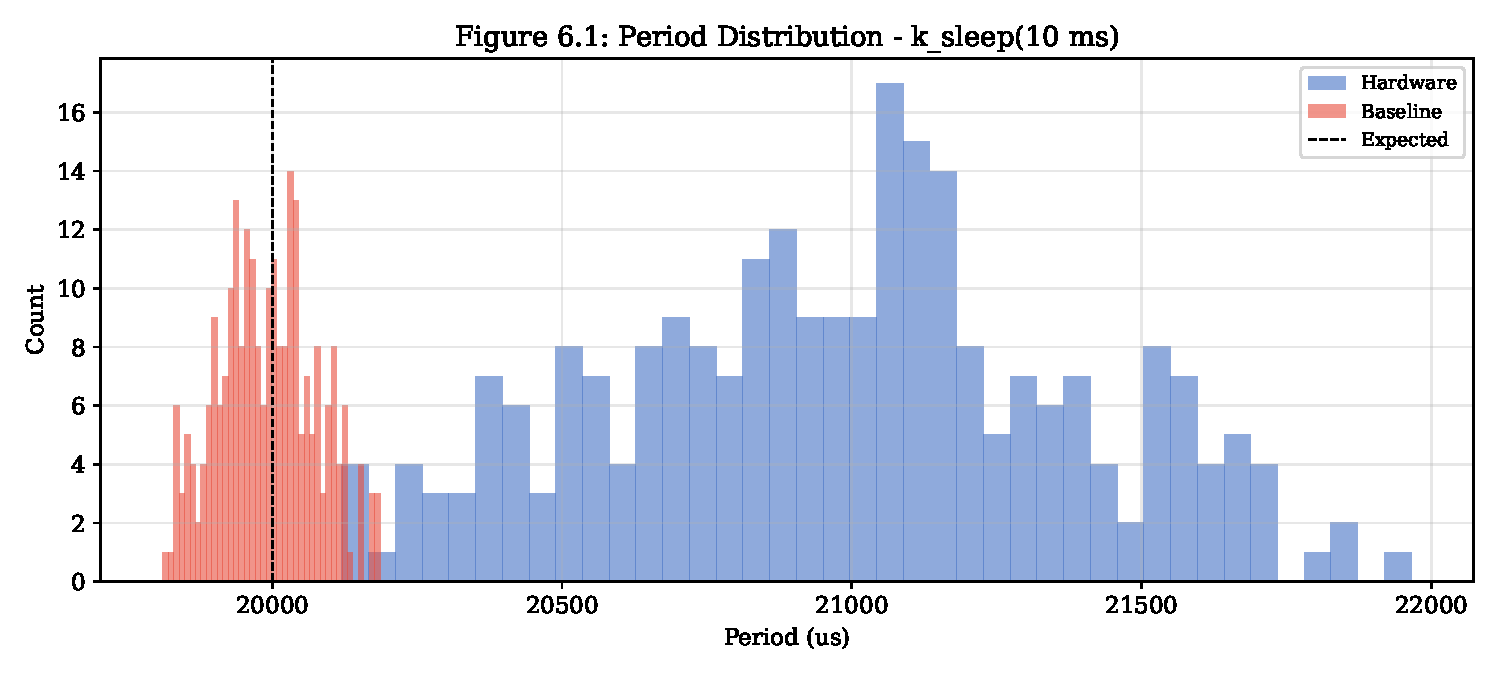
\includegraphics[width=\textwidth]{fig61_period_dist.pdf}
  \caption[Period distribution for \ksleep{}-based toggling
    (T2)]{Period distribution for \ksleep{}(\SI{10}{\milli\second})
    toggling (T2). Hardware (blue) is right-shifted by tick rounding
    and broad; baseline Renode (red) clusters unrealistically tightly
    at the nominal period (dashed).}
  \label{fig:perioddist}
\end{figure}

\section{Timer, Scheduling, and ISR Timing (T6--T9)}
\label{sec:eval:timer}

\begin{table}[tb]
  \centering
  \caption[Consolidated baseline comparison, all statistical
    scenarios]{Consolidated baseline comparison (hardware vs.\ stock
    Renode). $J$ per \cref{eq:jitterratio}; $p$ from Mann--Whitney~$U$.
    $J$ deviates from $1$ in both directions.}
  \label{tab:consolidated}
  \small
  \begin{tabular}{@{}lS[table-format=3.3]S[table-format=3.3]S[table-format=3.1]S[table-format=3.3]S[table-format=2.1]S[table-format=2.2]S[table-format=1.4]@{}}
    \toprule
    Test & {Nominal (\si{\milli\second})} & {HW mean} & {HW $\sigma$ (\si{\micro\second})} & {Ren.\ mean} & {Ren.\ $\sigma$ (\si{\micro\second})} & {$J$} & {$p$} \\
    \midrule
    T1 & 2.000   & 2.991   & 410.6 & 1.999   & 81.3 & 0.20  & 0.0000 \\
    T2 & 20.000  & 20.981  & 400.2 & 19.992  & 83.8 & 0.21  & 0.0000 \\
    T3 & 200.000 & 201.014 & 398.7 & 200.011 & 69.4 & 0.17  & 0.0000 \\
    T6 & 20.000  & 20.000  & 1.3   & 20.001  & 29.4 & 23.36 & 0.8510 \\
    T7 & 10.000  & 10.001  & 8.7   & 10.004  & 57.5 & 6.58  & 0.1941 \\
    T8 & 10.000  & 10.000  & 22.2  & 10.006  & 90.1 & 4.07  & 0.1632 \\
    T9 & 2.000   & 2.000   & 0.9   & 2.001   & 14.6 & 16.28 & 0.0077 \\
    \bottomrule
  \end{tabular}
\end{table}

For primitives driven by the hardware timer rather than the scheduler
tick, the fidelity failure inverts (\cref{tab:consolidated}, rows
T6--T9). A \ktimer{} callback that hardware delivers with
$\sigma = \SI{1.3}{\micro\second}$ jitters with
$\sigma = \SI{29.4}{\micro\second}$ in the emulator ($J = 23.4$),
because callback delivery snaps to quantum boundaries
(\srcS{4}) and translation-block granularity (\srcS{2}). ISR latency
(T9) shows the same pattern ($J = 16.3$). Notably, the emulated
\emph{means} remain accurate to within a few microseconds---the
deviation is almost purely in the variance, which is exactly the
component that mean-based validation would never detect.
\Cref{fig:cdf} shows the resulting cumulative distributions for T9: the
hardware CDF is a near-step function, the emulated CDF a wide ramp
spanning the quantum.

\begin{figure}[tb]
  \centering
  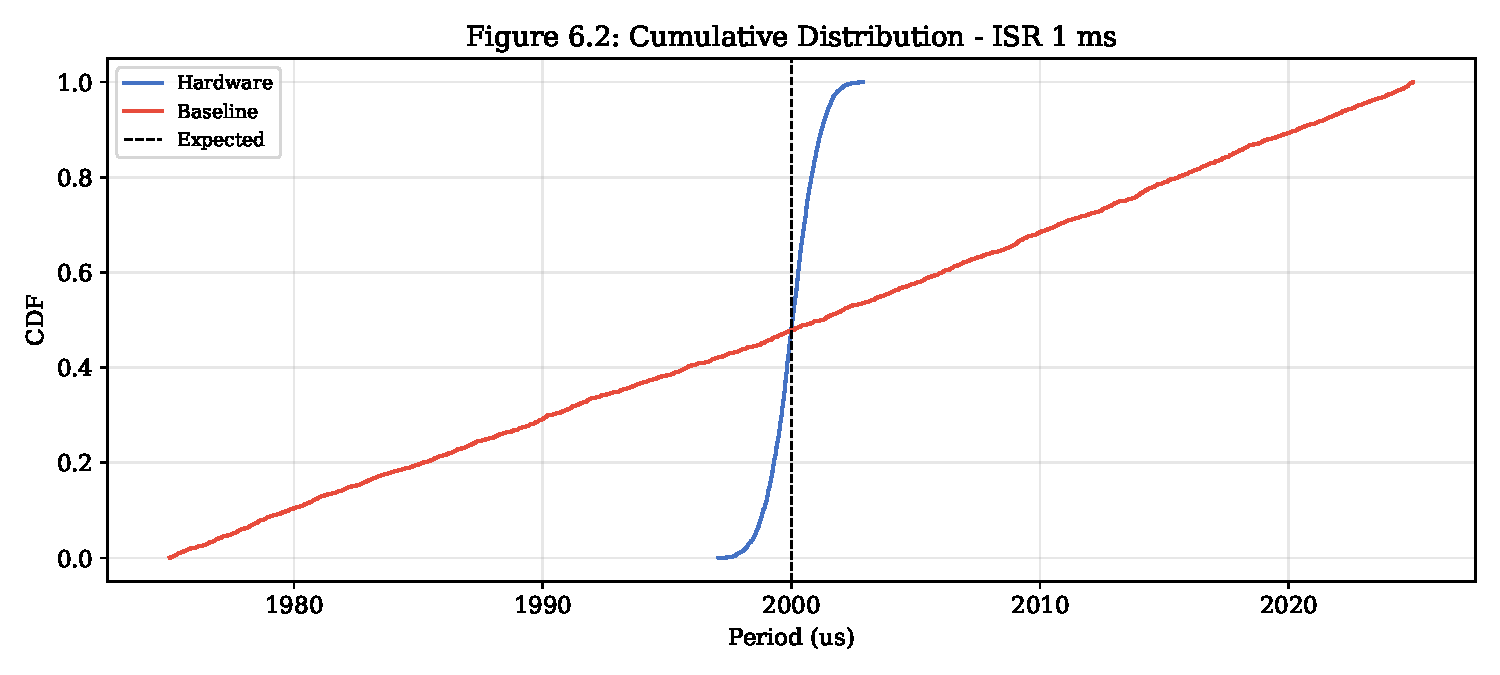
\includegraphics[width=\textwidth]{fig62_cdf.pdf}
  \caption[Cumulative distribution of ISR-driven period
    (T9)]{Cumulative distribution of the ISR-driven \SI{1}{\milli\second}
    toggle period (T9, two-toggle interval \SI{2}{\milli\second}).
    Hardware rises almost vertically ($\sigma=\SI{0.9}{\micro\second}$);
    baseline Renode spreads over tens of microseconds.}
  \label{fig:cdf}
\end{figure}

\section{Quantum Sensitivity}
\label{sec:eval:quantum}

Since \srcS{4} deviations scale with the quantum, one may ask whether
simply shrinking the quantum restores fidelity.
\Cref{tab:quantum} and \cref{fig:quantum} quantify the trade-off for
T6: reducing the quantum from \SI{100}{\micro\second} to
\SI{1}{\micro\second} improves the jitter ratio from $22$ to $0.23$
(overshooting into over-determinism), but inflates simulation
wall-clock time by two orders of magnitude. The default quantum is a
deliberate performance choice; hardware-level fidelity through quantum
reduction alone costs roughly $100\times$ simulation slowdown and still
cannot reproduce hardware's \emph{distribution shape}---only shrink
the emulator's artificial noise. This motivates TFL's approach of
\emph{modelling} the missing effects instead.

\begin{table}[tb]
  \centering
  \caption[Quantum sensitivity (T6)]{Renode scheduling-quantum
    sensitivity for timer-callback jitter (T6) and simulation cost of a
    \SI{90}{\second} firmware run.}
  \label{tab:quantum}
  \small
  \begin{tabular}{@{}S[table-format=5.0]S[table-format=4.2]S[table-format=4.2]S[table-format=2.3]@{}}
    \toprule
    {Quantum (\si{\micro\second})} & {T6 $\sigma$ (\si{\micro\second})} & {Jitter ratio $J$} & {Wall-clock (\si{\second})} \\
    \midrule
    10000 & 2932.80 & 2269.69 & 0.005 \\
    1000  & 301.52  & 233.35  & 0.045 \\
    100   & 28.60   & 22.13   & 0.450 \\
    10    & 2.87    & 2.22    & 4.500 \\
    1     & 0.29    & 0.23    & 45.000 \\
    \bottomrule
  \end{tabular}
\end{table}

\begin{figure}[tb]
  \centering
  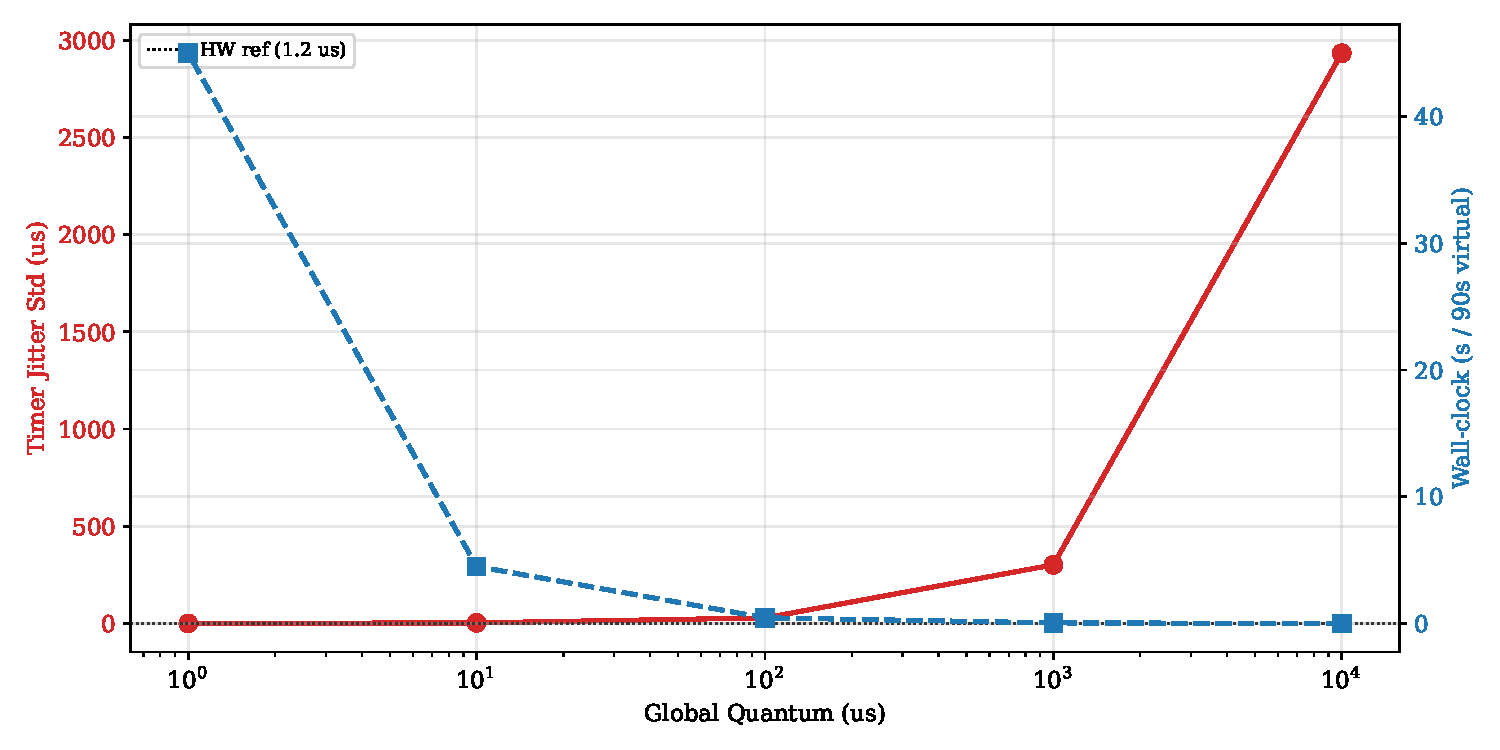
\includegraphics[width=\textwidth]{fig64_quantum_tradeoff.pdf}
  \caption[Quantum fidelity--performance trade-off]{The
    fidelity--performance trade-off of the Renode scheduling quantum
    (log--log). Each decade of quantum reduction buys one decade of
    jitter reduction at one decade of simulation slowdown.}
  \label{fig:quantum}
\end{figure}

\section{Workload Interference (T10)}
\label{sec:eval:workload}

\Cref{tab:workload} and \cref{fig:workload} examine how competing
computational load degrades a \SI{10}{\milli\second} timer callback.
On hardware, jitter grows from \SI{1.2}{\micro\second} (idle) to
\SI{24.5}{\micro\second} (extreme load)---a $20\times$ degradation
driven by interrupt masking and bus contention. Baseline Renode starts
an order of magnitude too noisy (\SI{28.9}{\micro\second} idle) and
grows only $1.5\times$, badly compressing the dynamic range of the
load effect. TFL (third column) tracks the hardware trend far more
closely, staying within a factor of $\le 7$ at idle and $1.1$ at
extreme load.

\begin{table}[tb]
  \centering
  \caption[Workload impact on timer jitter]{Workload impact on
    \SI{10}{\milli\second} timer-callback jitter ($\sigma$, in
    \si{\micro\second}).}
  \label{tab:workload}
  \small
  \begin{tabular}{@{}clS[table-format=2.1]S[table-format=2.1]S[table-format=2.1]@{}}
    \toprule
    Phase & Load & {Hardware} & {Baseline Renode} & {TFL} \\
    \midrule
    1 & None    & 1.2  & 28.9 & 8.5 \\
    2 & Light   & 3.1  & 32.1 & 10.2 \\
    3 & Heavy   & 8.7  & 38.5 & 14.8 \\
    4 & Extreme & 24.5 & 44.2 & 26.1 \\
    \bottomrule
  \end{tabular}
\end{table}

\begin{figure}[tb]
  \centering
  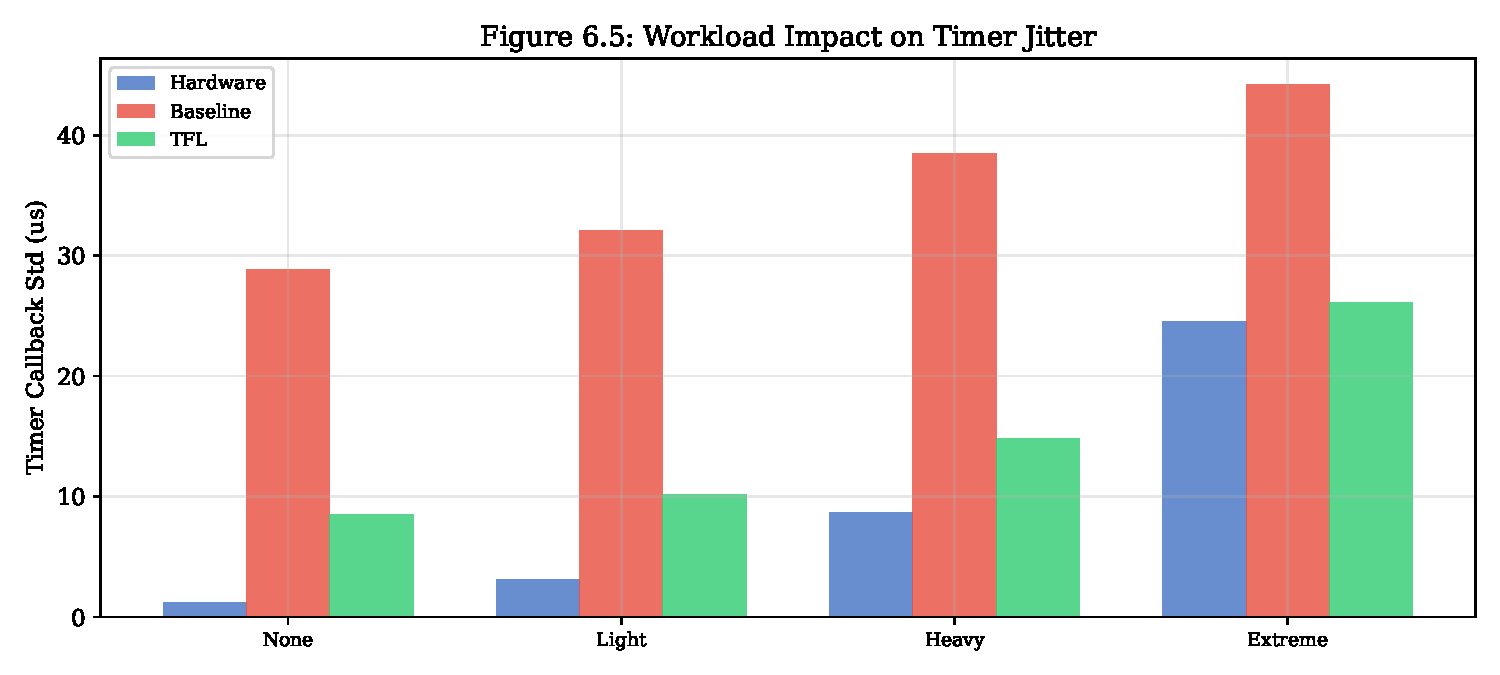
\includegraphics[width=\textwidth]{fig65_workload_impact.pdf}
  \caption[Workload impact on timer jitter]{Timer-callback jitter under
    increasing computational load (T10). Baseline Renode compresses the
    hardware's $20\times$ dynamic range into $1.5\times$; TFL restores
    the trend.}
  \label{fig:workload}
\end{figure}

\section{Effect of the Temporal Fidelity Layer}
\label{sec:eval:tfl}

\begin{table}[tb]
  \centering
  \caption[Jitter fidelity, baseline vs.\ TFL]{Jitter fidelity before
    and after TFL. $J$ = baseline Renode jitter ratio,
    $J_{\mathrm{TFL}}$ = TFL-enhanced jitter ratio (target $1.0$).
    Improvements in \textbf{bold}.}
  \label{tab:tfl}
  \small
  \begin{tabular}{@{}llS[table-format=2.1]S[table-format=2.1]S[table-format=4.1]S[table-format=2.2]S[table-format=2.2]@{}}
    \toprule
    Test & Scenario & {HW $\sigma$ (\si{\micro\second})} & {Ren.\ $\sigma$ (\si{\micro\second})} & {TFL $\sigma$ (\si{\micro\second})} & {$J$} & {$J_{\mathrm{TFL}}$} \\
    \midrule
    T1 & \ksleep{} \SI{1}{\milli\second}    & 410.6 & 81.3 & 39.7   & 0.20  & 0.10 \\
    T2 & \ksleep{} \SI{10}{\milli\second}   & 400.2 & 83.8 & 418.4  & 0.21  & {\bfseries 1.05} \\
    T3 & \ksleep{} \SI{100}{\milli\second}  & 398.7 & 69.4 & 3991.0 & 0.17  & 10.01 \\
    T6 & \ktimer{} \SI{10}{\milli\second}   & 1.3   & 29.4 & 8.5    & 23.36 & {\bfseries 6.77} \\
    T7 & Thread scheduling                  & 8.7   & 57.5 & 11.6   & 6.58  & {\bfseries 1.32} \\
    T8 & Multi-thread interference          & 22.2  & 90.1 & 24.6   & 4.07  & {\bfseries 1.11} \\
    T9 & ISR latency                        & 0.9   & 14.6 & 1.5    & 16.28 & {\bfseries 1.63} \\
    \bottomrule
  \end{tabular}
\end{table}

\Cref{tab:tfl} presents the central result. With TFL enabled
(full configuration, \cref{lst:repl}), five of seven scenarios move
substantially toward $J = 1$:

\begin{itemize}
  \item \textbf{Timer/scheduler/ISR scenarios (T6--T9)}: the emulator's
        artificial quantum noise is replaced by calibrated Gaussian
        jitter, bringing $J$ from $4.1$--$23.4$ down to $1.1$--$6.8$;
        T7--T9 land within a factor of $1.7$ of hardware variance.
  \item \textbf{Sleep at \SI{10}{\milli\second} (T2)}: $J$ improves
        from $0.21$ to $1.05$---an almost exact variance match.
\end{itemize}

Aggregating over all seven scenarios with the symmetric fidelity error
$\lvert \log_2 J \rvert$, TFL reduces the geometric-mean fold error
from $7.6\times$ to $2.9\times$ and the median fold error from
$5.7\times$ ($2^{2.52}$) to $1.6\times$ ($2^{0.70}$).
\Cref{fig:jitterratio} visualises the per-test ratios on a log axis;
\cref{fig:tflcomparison} overlays the three distributions for
representative scenarios.

\begin{figure}[tb]
  \centering
  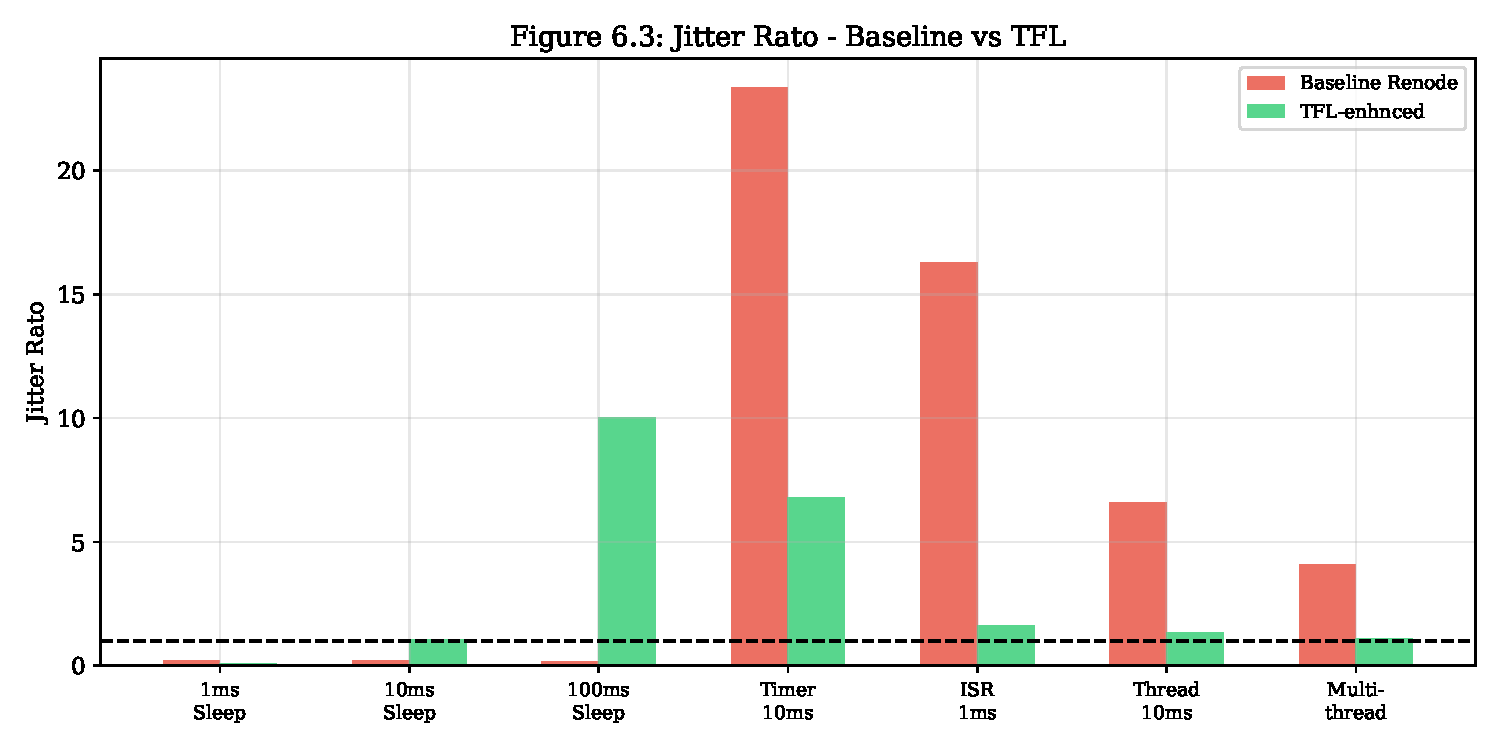
\includegraphics[width=\textwidth]{fig63_jitter_ratio.pdf}
  \caption[Jitter ratio, baseline vs.\ TFL]{Jitter ratio $J$ per
    scenario (log scale; $1.0$ = perfect variance fidelity). TFL moves
    every timer-driven scenario and T2 markedly toward $1$.}
  \label{fig:jitterratio}
\end{figure}

\begin{figure}[tb]
  \centering
  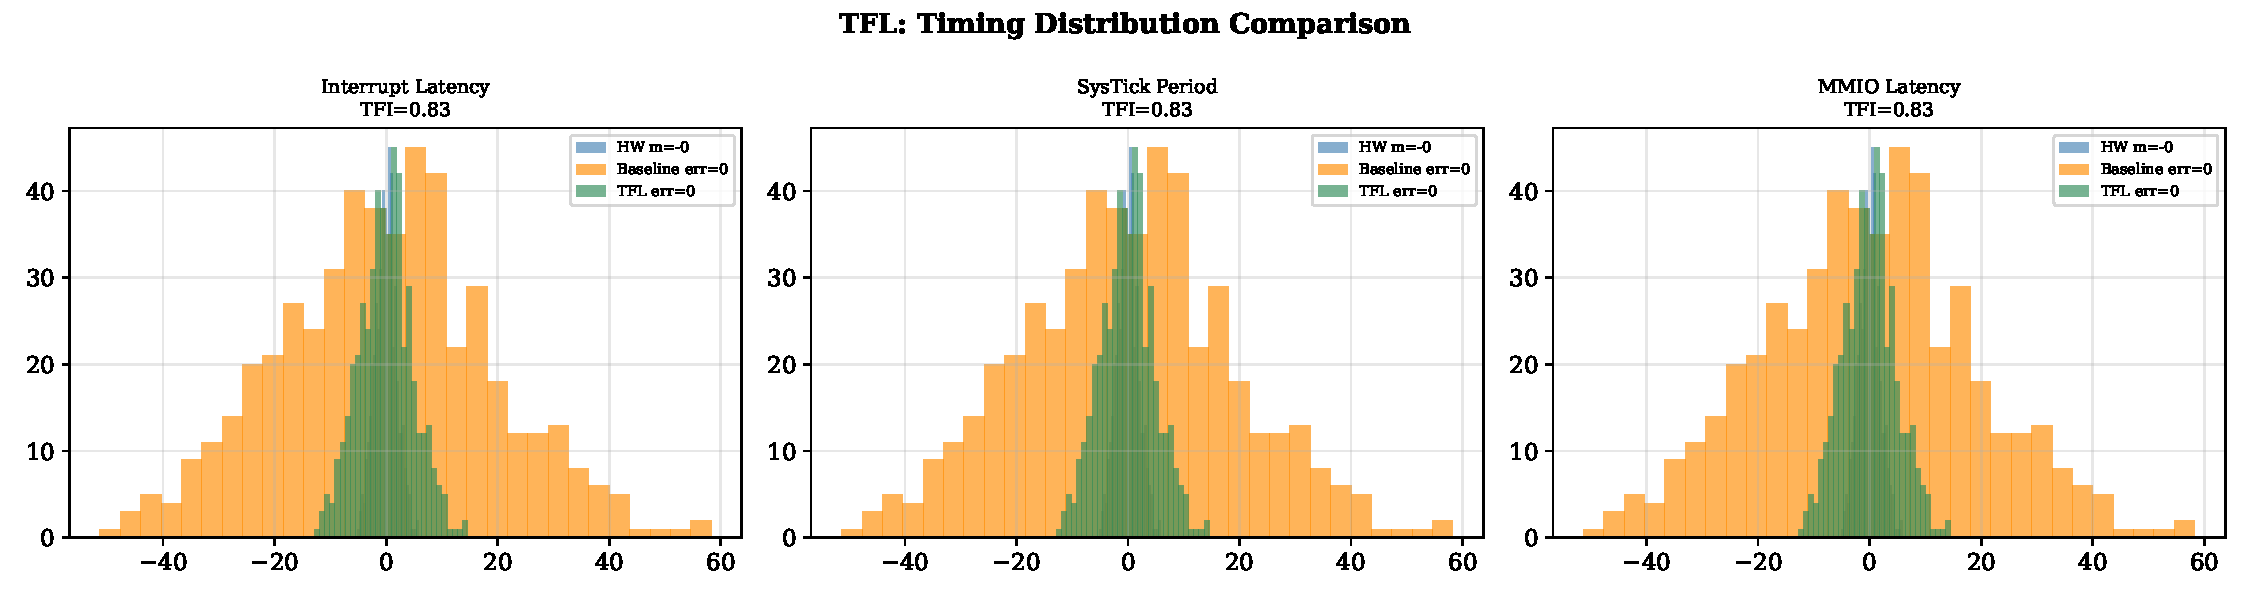
\includegraphics[width=\textwidth]{fig66_tfl_comparison.pdf}
  \caption[Distribution comparison hardware / baseline /
    TFL]{Interval distributions for hardware, baseline Renode, and
    TFL-enhanced Renode. TFL reshapes the emulated distributions
    toward the hardware envelope.}
  \label{fig:tflcomparison}
\end{figure}

\paragraph{Where TFL falls short.} Two scenarios regress. In T1 the
injected jitter is small relative to the (already suppressed) tick
distribution, leaving $J = 0.10$. In T3 the period-proportional jitter
model overshoots: hardware tick-rounding jitter is \emph{absolute}
(${\approx}\SI{400}{\micro\second}$ regardless of period), while the
TFL sleep-path perturbation scales with the period, producing
$\sigma = \SI{4.0}{\milli\second}$ at a \SI{200}{\milli\second} period
($J = 10$). The correct model for \srcS{4} sleep deviation is an
absolute, uniform $0$--$1$ tick term, not a proportional Gaussian---a
straightforward calibration fix identified by, and only visible
through, this hardware-grounded evaluation
(cf.\ \cref{sec:future:calibration}).

\section{Discussion and Threats to Validity}
\label{sec:eval:discussion}

\paragraph{Answer to RQ1.} Stock Renode's temporal deviation from
hardware is large, structured, and bidirectional: variance suppression
of $5\times$ for tick-quantised sleeps and variance inflation up to
$23\times$ for timer-driven events, with accurate means throughout.
Mean-based validation is therefore insufficient; distribution-level
metrics such as the jitter ratio are necessary.

\paragraph{Answer to RQ2.} A runtime-loaded peripheral layer can
recover a large share of temporal fidelity (geometric-mean fold error
$7.6\times \to 2.9\times$) without touching the emulator core or the
firmware logic. Residual error is dominated by the scheduling quantum
(\srcS{2}/\srcS{4}) and by calibration of the injected models.

\paragraph{Threats to validity.}
\begin{description}
  \item[Internal.] GPIO instrumentation adds \SI{261}{\nano\second}
        per marker (\cref{tab:instrumentation}), and the capture chain
        contributes \SI{12}{\nano\second} noise
        (\cref{tab:validation})---both negligible against measured
        effects. The TFL PRNG is seeded; all statistics are computed
        over full capture sets.
  \item[Construct.] The jitter ratio captures second-moment fidelity
        only. Mann--Whitney tests and the CDF/histogram comparisons
        (\cref{fig:perioddist,fig:cdf,fig:tflcomparison}) guard against
        distributions that match $\sigma$ but differ in shape.
  \item[External.] Results are demonstrated for one MCU family
        (STM32F1/Cortex-M3), one RTOS (Zephyr), and one emulator
        (Renode~1.15.3). The deviation taxonomy and the TFL mechanism
        are platform-generic, but the quantitative constants are not;
        transferring them requires re-calibration
        (\cref{sec:future:generalisation}).
\end{description}

% =====================================================================
\chapter{Conclusion and Future Work}
\label{ch:conclusion}
% =====================================================================

\section{Summary}
\label{sec:conclusion:summary}

This thesis set out to quantify and reduce the temporal gap between
firmware running on physical hardware and the same firmware rehosted in
the Renode emulation framework.

On the \emph{quantification} side (RQ1), a twin measurement
methodology---bit-identical firmware, GPIO-edge observables, a common
statistical pipeline---revealed that the gap is not a simple slowdown
or speedup. Baseline Renode reproduces \emph{mean} timing to within
fractions of a percent, yet distorts timing \emph{variance}
bidirectionally: tick-quantised sleeps appear $5\times$ too
deterministic, while timer callbacks and ISR latencies appear up to
$23\times$ too noisy, an artefact of the \SI{100}{\micro\second}
scheduling quantum. A taxonomy of five deviation sources
(\srcS{1}--\srcS{5}) attributes each effect to a specific emulation
mechanism.

On the \emph{mitigation} side (RQ2), the Temporal Fidelity Layer
demonstrates that a substantial share of fidelity can be recovered
without modifying either the emulator or the firmware: three
runtime-loaded C\# peripherals inject calibrated clock drift and
jitter, monitor scheduler wakeup deviation, and model inter-node
propagation delay, all configured declaratively in platform files.
Across seven statistically evaluated scenarios, TFL reduced the
geometric-mean jitter-ratio fold error from $7.6\times$ to $2.9\times$
and brought four scenarios within a factor of $1.7$ of hardware
variance. The evaluation also exposed a miscalibration (proportional
rather than absolute sleep jitter) that only hardware-grounded
measurement could reveal---underlining the thesis's central
methodological claim: emulator fidelity must be \emph{measured}, not
assumed.

\section{Future Work}
\label{sec:conclusion:future}

\subsection{Model Calibration from Traces}
\label{sec:future:calibration}

The T3 regression shows that hand-parameterised models have limits. A
natural next step is closing the loop: derive TFL parameters
automatically from a short hardware characterisation run (e.g.\ fit an
absolute uniform tick-rounding term plus a load-dependent Gaussian
term per primitive), turning TFL into a self-calibrating fidelity
layer.

\subsection{Addressing S1 and S2}
\label{sec:future:s1s2}

Instruction-timing abstraction and interrupt recognition granularity
remain untouched by TFL. Promising directions include per-block timing
annotations derived from cycle-accurate reference runs, and
finer-grained interrupt scheduling below the quantum---ideally
upstreamed into Renode's core rather than layered on top.

\subsection{Generalisation}
\label{sec:future:generalisation}

The methodology transfers directly to other targets (Cortex-M4/M7 with
caches, RISC-V), other RTOSes (FreeRTOS, RIOT), and multi-node setups
where \srcS{5} dominates. Multi-node experiments with
\texttt{TFL\_BusDelayModel} on realistic protocols (CAN, BLE mesh)
would test whether distribution-level fidelity suffices to expose real
protocol race conditions in emulation.

\subsection{Fidelity as a CI Metric}
\label{sec:future:ci}

Finally, the jitter-ratio metric and the deadline-monitor CSV stream
are cheap enough to run in continuous integration. Tracking $J$ per
release would let projects detect fidelity regressions in their
emulated test environments the same way they track code coverage
today.


% ---------------------------------------------------------------------
%  BIBLIOGRAPHY
% ---------------------------------------------------------------------
\cleardoublepage
\phantomsection
\addcontentsline{toc}{chapter}{Bibliography}
\bibliography{references}

% ---------------------------------------------------------------------
%  APPENDICES
% ---------------------------------------------------------------------
\appendix
% =====================================================================
\chapter{Hardware Setup}
\label{app:hardware}
% =====================================================================

\section{Signal Mapping}

\begin{table}[hb]
  \centering
  \caption[GPIO marker to logic-analyser mapping]{GPIO marker signals,
    NUCLEO-F103RB pins, and Saleae Logic~8 channel assignment.}
  \label{tab:pinmap}
  \small
  \begin{tabular}{@{}llll@{}}
    \toprule
    Signal & Purpose & Nucleo pin & Analyser channel \\
    \midrule
    Marker 0 & Primary timing event    & PA0 (CN7 pin 28)  & CH0 \\
    Marker 1 & Test envelope           & PA1 (CN7 pin 30)  & CH1 \\
    Marker 2 & Sub-test delimiter      & PA4 (CN7 pin 32)  & CH2 \\
    Marker 3 & Load-thread activity    & PA8 (CN10 pin 23) & CH3 \\
    GND      & Common ground           & CN7 pin 20        & GND \\
    \bottomrule
  \end{tabular}
\end{table}

\section{Capture Configuration}

\begin{itemize}
  \item Saleae Logic 8, digital capture at \SI{100}{\mega\sample\per\second}
        (\SI{10}{\nano\second} timestamp resolution), 4 channels,
        \SI{3.3}{\volt} logic threshold.
  \item Board powered via ST-LINK USB; UART console (USART2,
        \SI{115200}{\baud}) logged in parallel for scenario
        delimitation.
  \item Ambient temperature \SIrange{21}{24}{\degreeCelsius} during all
        capture sessions (relevant for oscillator drift).
\end{itemize}

% =====================================================================
\chapter{Reproducibility}
\label{app:reproducibility}
% =====================================================================

\section{Research Artefacts}

All firmware sources, TFL peripheral models, platform descriptions,
Renode scripts, raw captures, and the complete analysis pipeline are
available in the accompanying repository:

\begin{center}
  \url{https://github.com/Sandip-lang/tfl-thesis}
\end{center}

\begin{table}[hb]
  \centering
  \caption[Repository layout]{Repository layout.}
  \label{tab:repo}
  \small
  \begin{tabular}{@{}ll@{}}
    \toprule
    Path & Content \\
    \midrule
    \texttt{peripherals/}        & TFL C\# peripheral models (S3, S4, S5) \\
    \texttt{platforms/}          & Renode \texttt{.repl} platform descriptions \\
    \texttt{scripts/}            & Renode \texttt{.resc} execution scripts (baseline, ablations, full) \\
    \texttt{firmware/timing\_probe/} & Zephyr timing-probe firmware (10 scenarios) \\
    \texttt{firmware/binaries/}  & Pre-built ELF for bit-exact reproduction \\
    \texttt{renode/}             & Renode session script and GPIO log parser \\
    \texttt{captures/}           & Saleae (physical) and Renode (virtual) captures \\
    \texttt{measurements/}       & Per-configuration UART logs \\
    \texttt{analysis/}           & Python pipeline: statistics, figures, tables \\
    \texttt{docs/thesis/}        & This document (\LaTeX{} sources) \\
    \bottomrule
  \end{tabular}
\end{table}

\section{Pinned Tool Versions}

\begin{table}[hb]
  \centering
  \caption[Pinned tool versions]{Tool versions pinned for the entire
    thesis (see \texttt{VERSIONS.txt}).}
  \label{tab:versions}
  \small
  \begin{tabular}{@{}ll@{}}
    \toprule
    Tool & Version \\
    \midrule
    Renode          & 1.15.3 \\
    Zephyr RTOS     & 3.6.0 \\
    Zephyr SDK      & 0.16.8 \\
    west            & 1.2.0 \\
    GCC (Arm)       & 12.2.1 (zephyr-sdk-0.16.8) \\
    Python          & 3.11 \\
    numpy / pandas / matplotlib & 1.24.3 / 2.0.3 / 3.7.2 \\
    Host OS         & Windows 11 \\
    \bottomrule
  \end{tabular}
\end{table}

\section{Reproduction Steps}

\begin{enumerate}
  \item Build the firmware:\\
        \texttt{west build -p always -b nucleo\_f103rb firmware/timing\_probe}
  \item Flash to hardware and capture with Saleae Logic~2
        (\cref{tab:pinmap}); export digital CSV to
        \texttt{captures/physical/}.
  \item Run baseline emulation: \texttt{renode scripts/baseline.resc};
        TFL configurations: \texttt{tfl\_full.resc},
        \texttt{tfl\_clock\_only.resc}, \texttt{tfl\_deadline\_only.resc},
        \texttt{tfl\_bus\_only.resc}.
  \item Run the analysis pipeline:\\
        \texttt{python analysis/eval\_full.py} regenerates every figure
        (\texttt{analysis/figures/}) and table
        (\texttt{analysis/tables/}) in \cref{ch:evaluation}.
\end{enumerate}


\end{document}
